\documentclass{article}
\usepackage[UKenglish]{babel}
\usepackage[UKenglish]{isodate}
\usepackage{fullpage}
\usepackage{graphicx}
\usepackage{hyperref}
\usepackage{listings}

\title{Automated Benchmarking of Container Applications}
\author{Paulius Dilkas}

\begin{document}
\maketitle

%\begin{abstract}
%\end{abstract}

\section{Introduction}

% Motivation
% OpenShift, MiniShift
% Prometheus
% Flink

\section{Architecture}

% components.yaml

% global.yaml

\subsection{Software Architecture}

% classes

% Makefile

% experiment.py

\subsection{Software Configuration}

Added to the Flink configuration file (\texttt{flink-conf.yaml}):
\begin{lstlisting}
metrics.latency.interval: 1000
metrics.reporters: prom
metrics.reporter.prom.class: org.apache.flink.metrics.prometheus.PrometheusReporter
metrics.reporter.prom.port: 9250
\end{lstlisting}

Prometheus is configured as follows (\texttt{prometheus.yml}):
\begin{lstlisting}
global:
  scrape_interval:     1s
  evaluation_interval: 1s

scrape_configs:
  - job_name: 'benchmarker'
    static_configs:
      - targets: ['jobmanager:9250', 'taskmanager:9250']
\end{lstlisting}

Modified the configuration file of the Prometheus add-on for
MiniShift\footnote{\url{https://github.com/minishift/minishift-addons/tree/master/add-ons/prometheus}}
to disable OAuth-based authentication by replacing
\texttt{-skip-auth-regex=\^{}/metrics} with \texttt{-skip-auth-regex=\^{}/}.
% write about the implications of this hack

% Disabled Prometheus OAuth authentication

\section{Docker and OpenShift}

Two simple Dockerfiles were created.

Control pod entrypoint:
\begin{lstlisting}
#!/bin/sh

flink run -m jobmanager:8081 benchmarker-0.1.jar &
java -cp benchmarker-0.1.jar ControlServer
\end{lstlisting}

% docker-compose.yml

% -> OpenShift manifestos

\section{Local Performance Tuning}

\subsection{Experiments}

\begin{figure}
  \centering
  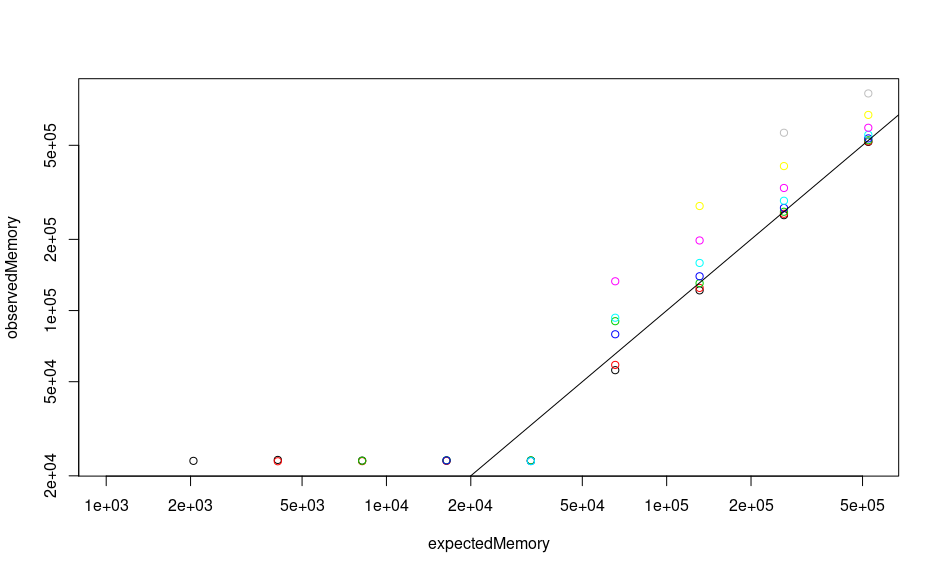
\includegraphics[width=\textwidth]{../proof_of_concept/comparison1.png}
  \caption{}
  \label{}
\end{figure}

\begin{figure}
  \centering
  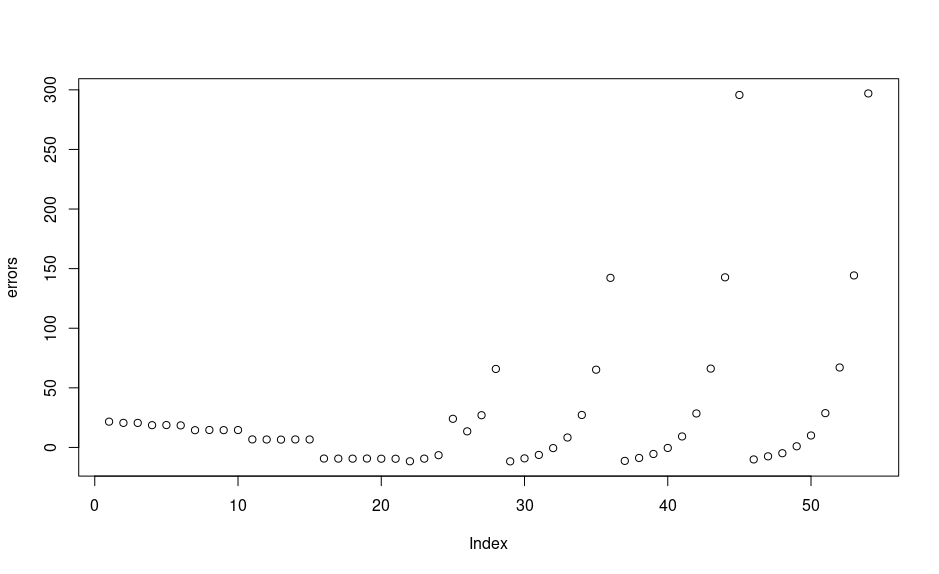
\includegraphics[width=\textwidth]{../proof_of_concept/comparison2.png}
  \caption{}
  \label{}
\end{figure}

\subsection{Adjusted Performance}

\begin{figure}
  \centering
  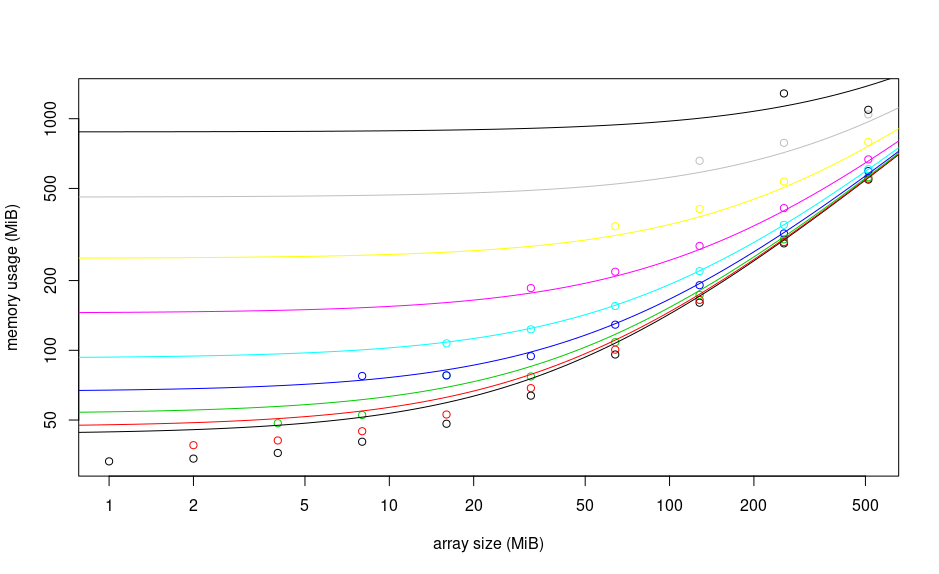
\includegraphics[width=\textwidth]{../proof_of_concept/prediction1.png}
  \caption{}
  \label{}
\end{figure}

\begin{figure}
  \centering
  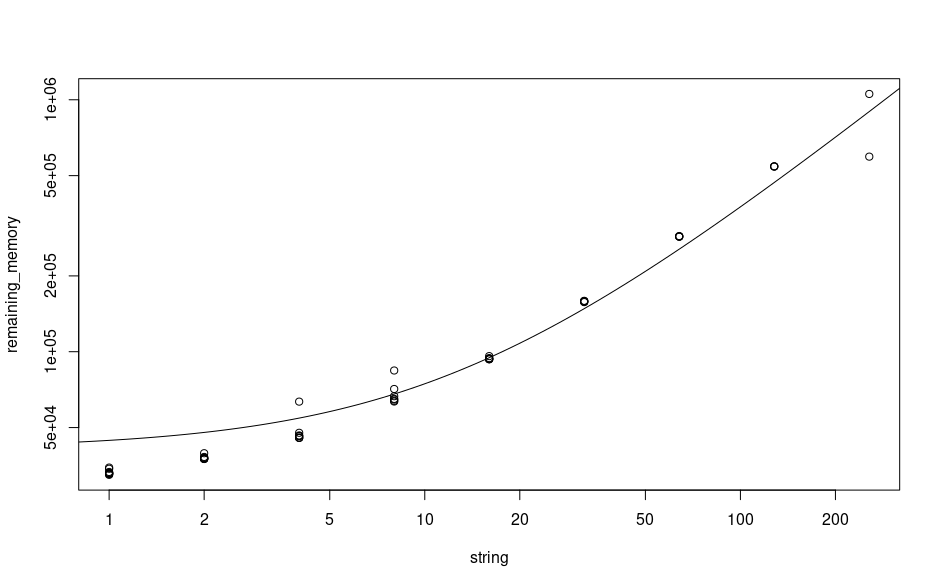
\includegraphics[width=\textwidth]{../proof_of_concept/prediction2.png}
  \caption{}
  \label{}
\end{figure}

\section{Experimental Results}

\section{Conclusion}

\end{document}